% Template for ICASSP-2013 paper; to be used with:
%          spconf.sty  - ICASSP/ICIP LaTeX style file, and
%          IEEEbib.bst - IEEE bibliography style file.
% --------------------------------------------------------------------------



% ++++++++++++++++++++++++++++++++++++++++++++++++++++++++++++++++++++++++++++++
% + Document preamble
\documentclass{article}


% Packages
% --------
\usepackage{spconf,amsmath,graphicx}
\usepackage[total={178mm,229mm},top=25mm,left=19mm]{geometry}
\usepackage{amssymb}
\usepackage{amsthm}
\usepackage{bm}
\usepackage[font=small,labelfont=bf]{caption}
\usepackage{subcaption}
\usepackage{cite}
\usepackage{soul}
\usepackage{algorithm}
\usepackage{algorithmic}

% Definitions
% -----------
\def\x{{\bm x}}
\def\hx{\hat{x}}
\def\bhx{\bm{\hat{x}}}
\def\y{{\bm y}}
\def\z{{\bm z}}
\def\e{{\bm e}}
\def\n{{\bm n}}
\def\A{{\bm A}}
\def\D{{\bm D}}
\def\F{{\bm F}}
\def\I{{\bm I}}
\def\L{{\cal L}}
\def\N{{\mathbb N}}
\def\R{{\mathbb R}}
\def\C{{\mathbb C}}


% Mathematical tips
% -----------------
\providecommand{\abs}[1]{\lvert#1\rvert}
\providecommand{\norm}[1]{\lVert#1\rVert}
\renewcommand{\Re}[1]{\mathfrak{Re}\lbrace#1\rbrace}
\renewcommand{\Im}[1]{\mathfrak{Im}\lbrace#1\rbrace}
\providecommand{\sinc}{\text{sinc}}
\providecommand{\DFT}[1]{\text{DFT}\lbrace#1\rbrace}
\providecommand{\e}[1]{\text{e}^{#1}}
\renewcommand{\d}{\text{d}}
\providecommand{\toe}[2]{\text{Toe}_{#2}\,\lbrace#1\rbrace}
\newtheorem{prop}{Proposition}
\newtheorem{remark}{Remark}


% - end of document preamble
% ------------------------------------------------------------------------------



% ++++++++++++++++++++++++++++++++++++++++++++++++++++++++++++++++++++++++++++++
% + Beginning of content
\begin{document}
%\ninept


% Title, authors and address
% --------------------------
\title{Finite dimensional FRI}

\name{Jon O\~{n}ativia$\,^\dagger$, Yue M. Lu$\,^\star$ and Pier Luigi Dragotti$\,^\dagger$
\thanks{This work was supported by the European Research Council (ERC)
starting investigator award Nr. 277800 (RecoSamp).}}
\address{$^\dagger$ Communications and Signal Processing Group (CSP),
Imperial College London, UK\\
\normalsize \texttt{\{ jon.onativia, p.dragotti \} @imperial.ac.uk}\\ \\
$^\star$ Signals, Information, and Networks Group (SING), Harvard University, USA\\
\normalsize \texttt{yuelu@seas.harvard.edu}
}

\maketitle




% ---------------------
% Abstract and keywords
% ---------------------
\begin{abstract}
Traditional Finite Rate of Innovation (FRI) theory has considered the problem of sampling 
continuous-time signals. This framework can be naturally extended
to the case where the input is a discrete-time signal. Here we present a novel approach 
which uses both the traditional FRI sampling scheme, based on the annihilating filter method, 
and the fact that in this new setup the null space of the problem to be 
solved is finite dimensional. 

In the noiseless scenario, we show that this new approach is able to perfectly recover the 
original signal at the critical sampling rate. We also present simulation results in the noisy scenario
where this new approach improves performances in terms of the mean squared error (MSE) of the 
reconstructed signal when compared to the canonical FRI algorithms and compressed sensing (CS).
\end{abstract}

\begin{keywords}
Finite rate of innovation, sampling theory, sparsity,
annihilating filter.
\end{keywords}




% ------------
% Introduction
% ------------

\section{Introduction}
\label{sec:intro}


FRI sampling theory \cite{vetterli2002,blu2008,berent2010,tur2011} has shown that it is possible to sample
and reconstruct classes of non-bandlimited signals.
Streams of Diracs are the canonical example of FRI signals. They are not bandlimited but 
are sparse in time and have a finite number of degrees of freedom per unit of time, which is 
known as the rate of innovation. The final goal of FRI methods is to retrieve the exact 
location and amplitude of the Diracs from a set of samples. 
In the continuous-time setup, the signal is filtered and then sampled in order to obtain a 
discrete sequence.
In \cite{vetterli2002} the signal is filtered using the sinc kernel. Authors 
in \cite{dragotti2007} present the use of polynomial or exponential reproducing kernels with
the advantage of achieving perfect reconstruction with compact support kernels. 
This framework has recently been extended to arbitrary sampling kernels with the penalty of 
not achieving perfect reconstruction \cite{uriguen2013}. 
To some extent, these methods are all based on the fact that 
the Fourier transform of a sum of Diracs is given by a sum of exponentials.
%and the various sampling schemes
%provide some measurements that are related to some of the coefficients of the Fourier transform. 
The reconstruction is then based on estimating exponentials from a sequence of samples, which is a 
classical problem in spectral estimation \cite{rao1992,stoica2005}. 

This framewok can be naturally extended to discrete-time signals. In this case, the sampling 
process can be modelled with a matrix multiplication. The input signal is given by a high dimensional
vector with few non-zero elements. The acquired signal is a vector of lower dimension which is given 
by the product of a fat matrix with the input signal. Note that since the acquisition matrix is fat, 
the dimension of its null space is strictly positive. 
The goal is to reconstruct the sparse input vector from the acquired samples. 
%The solution is not unique, since the system of equations is 
%underdetermined. In other words, the null space of the acquisiton matrix is nonempty.
Some preliminary work has already been published where the FRI framework is applied in the 
discrete-time setup \cite{hormati2007} and is compared to $\ell_1$--minimization techniques,
which is the traditional reconstruction approach in the compressed sensing (CS) framework \cite{donoho2006,candes2006}.
In this paper we present a novel method that is based on the annihilating filter 
that is used in the traditional FRI framework, but we take advantage of the fact that 
in this new context the null space has finite dimension. 
The annihilating method requires a root finding 
step that becomes unstable in high noise scenarios. This new approach avoids this root finding step. 
We show simulation results where the new finite dimensional FRI method outperforms traditional FRI and CS.

In Section \ref{sec:annihil} we describe the annihilating filter method which is inherently valid for 
the continuous-time and the discrete-time cases. If the input signal is discrete, 
the solution is mapped to a discrete time grid. In Section \ref{sec:finite_fri} we present 
our new approach, we first establish the uniqueness of the solution in the noiseless case, 
we then present an extension of the algorithm when noise is present.
In Section \ref{sec:results} we present simulation results and then conlude
in Section \ref{sec:conclusions}.




% --------------
% Second section
% --------------

\section{Traditional FRI in discrete-time}
\label{sec:annihil}

Let $\x \in \C^N$ be a discrete time signal formed by a stream of $K$ Diracs. 
The expression in time is given by

\begin{equation}
x[n] = \sum_{k=1}^K a_k \, \delta [n - n_k], \qquad n = 0, 1, \ldots, N-1,
\label{eq:sparse_x}
\end{equation}

\noindent
where $n_k \in [0,N-1]$ and $a_k \in \C \setminus \{0\}$, for $1 \leq k \leq K$,
are unknown integer delays and complex valued amplitudes, respectively. We assume that 
all delays are distinct and therefore the signal $\x$ has $2K$ degrees of freedom. 
Let us also assume that we have access to $M<N$ coefficients of the unitary discrete Fourier transform 
(DFT) of $\x$. We can express the sampling process in matricial form as follows

\begin{equation}
\y = \D \, \x,
\label{eq:under_y}
\end{equation}

\noindent 
where $\y \in \C^M$ are the available samples and $\D \in \C^{M \times N}$ is a partial Fourier matrix:
%$\left( \D \right)_{m,n} = \tfrac{1}{\sqrt{N}} \, e^{-j \,\tfrac{2\pi}{N}\,m\,n}$,
$\left( \D \right)_{m,n} = \exp \left(-j2\pi mn/N\right) / \sqrt{N}$,
with $m=0,\ldots,M-1$ and $n=0,\ldots,N-1$.

The unitary DFT of $\x$, denoted by $\bhx \in \C^N$, consists of the sum of $K$ exponentials

\begin{equation}
\hx[m] = \tfrac{1}{\sqrt{N}} \sum_{k=1}^K a_k \, e^{-j \omega_k m}, \qquad m = 0, 1, \ldots, N-1,
\label{eq:X_k}
\end{equation}

\noindent
where $\omega_k = \tfrac{2\pi}{N}\,n_k$. The annihilating filter $h[m]$ is a $K+1$ taps
filter such that $(\hx * h)[m] = 0$. The $z$-transform of $h[m]$ is given by
$H(z) = \sum_{m=0}^{K} h[m] \, z^{-m} = \prod_{k=1}^{K} \left(1-u_k \, z^{-1}\right)$,
where $u_k = e^{-j\omega_k}$.
$H(z)$ is a polynomial of order $K$ in the complex variable $z$ with roots at $z=u_k$, 
that is, $H(z)\vert_{z=u_k}=0$. Note that the $K$ roots are distinct and non-zero, we thus 
always have that $h[0] \neq 0$ and $h[K] \neq 0$.
It can easily be shown that the sequence $\hx[m]$ is annihilated by this filter:

\begin{equation}
\begin{aligned}
(\hx * h)[m] 
& = \sum_{l=0}^{K} \hx[m-l] \, h[l] \\
& = \tfrac{1}{\sqrt{N}} \sum_{l=0}^{K} \sum_{k=1}^K a_k \, u_k^{m-l} \, h[l] \\
& = \tfrac{1}{\sqrt{N}} \sum_{k=1}^{K} a_k \, u_k^{m} 
    \, \underbrace{\left(\sum_{l=0}^{K} h[l] \, u_k^{-l}\right)}_{H(z)\vert_{z=u_k}}
  = 0.
\end{aligned}
\end{equation}
 
 The annihilating filter method consists of finding the filter coefficients 
 $\left(h[m]\right)_{m=0}^K$, and estimating the frequencies $\omega_k$ from 
 the roots of the polynomial $H(z)$. The filter can be obtained by solving the 
 following linear system

\begin{equation}
\begin{bmatrix}
\hx[K] & \hx[K-1] & \ldots & \hx[0]\\
\hx[K+1] & \hx[K] & \ldots & \hx[1]\\
\vdots & \vdots & \ddots & \vdots\\
\hx[2K] & \hx[2K-1] & \ldots & \hx[K]\\
\end{bmatrix}
\,
\begin{bmatrix}
h[0]\\ h[1]\\ \vdots\\ h[K]
\end{bmatrix}
= 0
\label{eq:system}
\end{equation}

It can be shown that if the coefficients $\hx[k]$ satisfy \eqref{eq:X_k},
the Toeplitz matrix in \eqref{eq:system} has rank $K$ \cite{maravic2005}. Thus, the system
has a unique solution up to an amplitude factor. If we impose $h[0]=1$ we can 
drop a row of the system and find the unique solution from only $2K$ 
consecutive values of $\hx[k]$. 
From the knowledge of $\omega_k$, and since coefficients $\hx[k]$ are linear in $a_k$,  
the amplitudes $a_k$ are computed from $K$ samples of \eqref{eq:X_k}.

This approach is able to perfectly reconstruct the $K$-sparse signal $\x$
from only $2K$ coefficients of the DFT of $\x$, but requires a nonlinear 
step to find the roots of the annihilating filter. These can be obtained from the 
eigenvalues of the companion matrix. 
There exist an alternative approach \cite{maravic2005} that do not involve root 
finding and is based on the 
matrix pencil method \cite{hua1990}. It is in essence based on the same principle
that is used in the ESPRIT algorithm \cite{paulraj1985} for
the estimation of directions of arrival of signals in arrays of
antennas. This approach does not explicitly find 
the roots of a polynomial, but involves solving a generalized eigenvector problem 
and presents similar performances.

In what follows we present a new linear approach for FRI signal reconstruction. The
proposed method is also based on the annihilating filter method, 
but it takes advantage of the fact that the underlying vector $\x$ is finite 
dimensional.




% -------------
% Third section
% -------------

\section{Finite dimensional FRI: new approach}
\label{sec:finite_fri}

In the previous section we have shown that we can compute the annihilating filter coefficients 
if the number of available samples $M$ is greater than or equal to $2K$.
In this section we assume that the coefficients of the annihilating filter have already been computed, but
we want to avoid the root finding step.
We now present an algebraic approach to reconstructing the $K$-sparse vector $\x$.


\subsection{Perfect reconstruction in the noiseless scenario}

Equation \eqref{eq:under_y}, where $\x$ is unknown, is an underdetermined system and therefore the solution
is not unique. Among all the possible solutions we want to find the one that is $K$-sparse.

\begin{prop}
Let $\x \in \C^{N}$ and $\y \in \C^{M}$ be given as in \eqref{eq:sparse_x} and \eqref{eq:under_y}
respectively. If $M \geq 2K$ the solution to 
\eqref{eq:under_y} is unique and can be found by solving two linear inversions.
\label{prop}
\end{prop}

\begin{proof}
Since $M\geq2K$, we estimate $\bm{h}$ from \eqref{eq:system} but now we do not compute its roots.
We have that $\D$ is of full rank $M$, since it is obtained from the first $M$ rows of the 
Fourier matrix $\F_N$. Using the pseudoinverse $\D^\dagger$, we can retrieve $\x$ up to 
the null space of $\D$. Note that since $\F_N$ is an orthogonal matrix, that is 
$\F_N \, \F_N^H = \F_N^H \, \F_N = \I_M$, the pseudoinverse of $\D$ is directly $\D^H$,
where the superscript $^H$ denotes the Hermitian transpose of a matrix.
We can therefore write

\begin{equation}
\x = \D^H \, \y + \sum_{l=1}^{L} \beta_l \, \n_l
\label{eq:null_space}
\end{equation}

\noindent
where $\beta_l$ are unknown coefficients, $L=N-M$ is the size of the null space 
and $\n_l$ are $L$ orthonormal vectors that span the 
null space of $\D$, that is $\n_l \in N(\D)$ where 
$N(\D) = \lbrace \n \in \C^M \,\vert\, \D \, \n = \bm{0} \rbrace$. The natural choice for $\n_l$, 
$l=1,\ldots,L$, is to pick the last $N-M$ columns of $\F_N^H$. If we premultiply equation 
\eqref{eq:null_space} by $\F_N$ we obtain the Fourier transform of $\x$

\begin{equation}
\bhx = \F_N \, \x = \F_N \, \D^H \, \y + \sum_{l=1}^{L} \beta_l \, \F_N \, \n_l.
\label{eq:x_k_null_space}
\end{equation}

\noindent
It can easily be verified that $\F_N \, \D^H = \begin{bmatrix} \I_M \\ \bm{0}_{L,M} \end{bmatrix}$
and $\F_N \, \n_l = \e_{M+l}$, where $\e_i$ is the $i$-th vector of the canonical basis. 
Note that coefficients $\beta_l$ are exactly the missing coefficients of the Fourier transform of $\x$.
Let define $\z = \F_N \, \D^H \, \y$. 

Let $\bm{S} \in \C^{(N-K)\times(K+1)}$ be the Toeplitz matrix where the first row is given 
by coefficients $\hx[K], \hx[K-1], \ldots, \hx[0]$ and the first column by 
$\hx[K], \hx[K+1], \ldots, \hx[N-1]$. Note that $\bm{S}$ is fully specified by vector $\bhx$.
In what follows, we denote by $\toe{\cdot}{K}$ the operation of building the $(N-K)\times(K+1)$
Toeplitz matrix from a $N \times 1$ vector in the way we define matrix $\bm{S}$.
Since the $N$ coefficients $\hx[k]$ satisfy \eqref{eq:X_k}, the annihilating filter's system from 
\eqref{eq:system} is also satisfied:

\begin{equation}
\bm{S} \, \bm{h} = \bm{0}.
\label{eq:compact_sys}
\end{equation}

If we replace the Fourier transform of $\x$ with the expression obtained in \eqref{eq:x_k_null_space},
matrix $\bm{S}$ can be expressed as

\begin{equation}
\bm{S} = \bm{Z} + \sum_{l=1}^{L} \beta_l \, \bm{E}_{M+l},
\label{eq:S}
\end{equation}

\noindent
where $\bm{Z} = \toe{\z}{K}$ and $\bm{E}_i = \toe{\bm{e}_i}{K}$. We then replace \eqref{eq:S} in 
\eqref{eq:compact_sys}, and given that $\bm{h}$ is known, we can turn the system of 
equations in a new problem with $L$ unknowns:

\begin{equation}
\begin{bmatrix}
\bm{E}_{M+1} \, \bm{h} & \ldots & \bm{E}_{N} \, \bm{h}
\end{bmatrix}
\,
\begin{bmatrix}
\beta_1\\
\vdots\\
\beta_L
\end{bmatrix}
=
- \bm{Z} \, \bm{h}.
\label{eq:system_beta}
\end{equation}

The first $M-K$ rows of this system are trivially equal to zero because matrices $\bm{E}_{M+l}$
are all zero in these rows and rows of $\bm{Z}\,\bm{h}$ are also equal to zero because
they contain the convolution of exactly $K+1$ consecutive coefficients of $\bhx$ with 
the annihilating filter.  
Let define $\A$ as the remaining $N-M$ rows of matrix 
$\begin{bmatrix} \bm{E}_{M+1} \, \bm{h} & \ldots & \bm{E}_{N} \, \bm{h} \end{bmatrix}$.
Matrix $\A$ is of size $L\times L$ and is given by

\begin{equation}
\bm{A} = 
\begin{bmatrix}
h[0]   & 0      & \ldots & \ldots & \ldots & 0      & 0      \\
h[1]   & h[0]   & \ldots & \ldots & \ldots & 0      & 0      \\
\vdots & \ddots & \ddots &        &        & \vdots & \vdots \\
h[K]   & \ldots & h[1]   & h[0]   & \ldots & 0      & 0      \\
\vdots & \vdots & \ddots &        & \ddots & \ddots &        \\
0      & 0      & \ldots & h[K]   & \ldots & h[1]   & h[0]   \\
\end{bmatrix}.
\end{equation}

This is a lower triangular matrix where all the elements in the main diagonal are
non-zero. Moreover, we have imposed $h[0]=1$ when computing the annihilating filter,
thus, the elements of the main diagonal are all equal to one. Matrix $\bm{A}$
has therefore rank $N-M$ and the system has a unique solution. 

\end{proof}

\begin{figure}[t]
\centering
\begin{subfigure}{.22\textwidth}
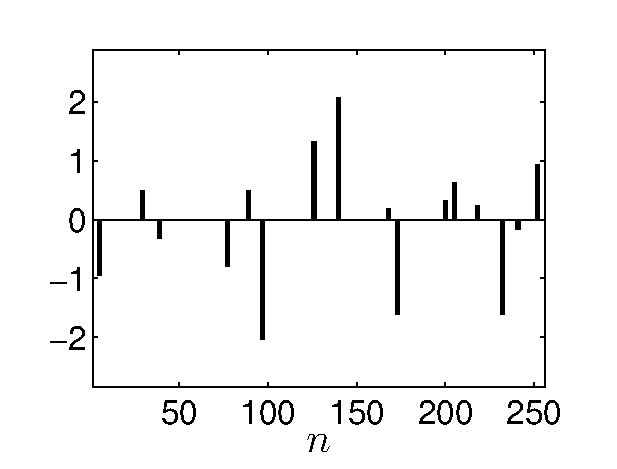
\includegraphics[width=\linewidth]{figures/signal_M_256_K_16}
\caption{Original signal $\x$}
\end{subfigure}
\begin{subfigure}{.22\textwidth}
%\includegraphics[width=\linewidth]{figures/ft_signal_M_256_K_16}
%\caption{Real part of $\bhx[k]$}
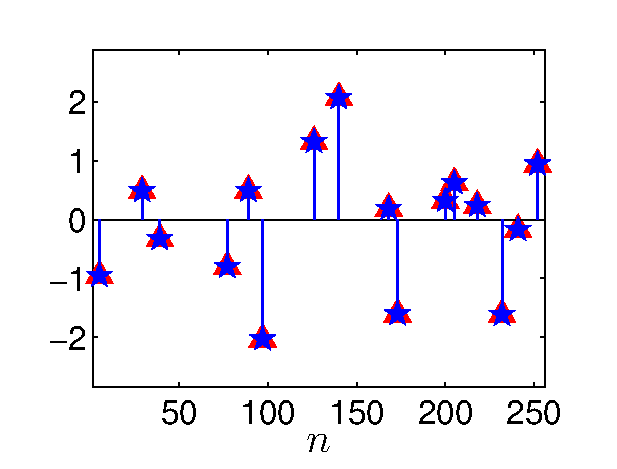
\includegraphics[width=\linewidth]{figures/signal_reconstr_M_256_N_32_K_16}
\caption{Reconstructed signal}
\end{subfigure}
\\
\begin{subfigure}{.44\textwidth}
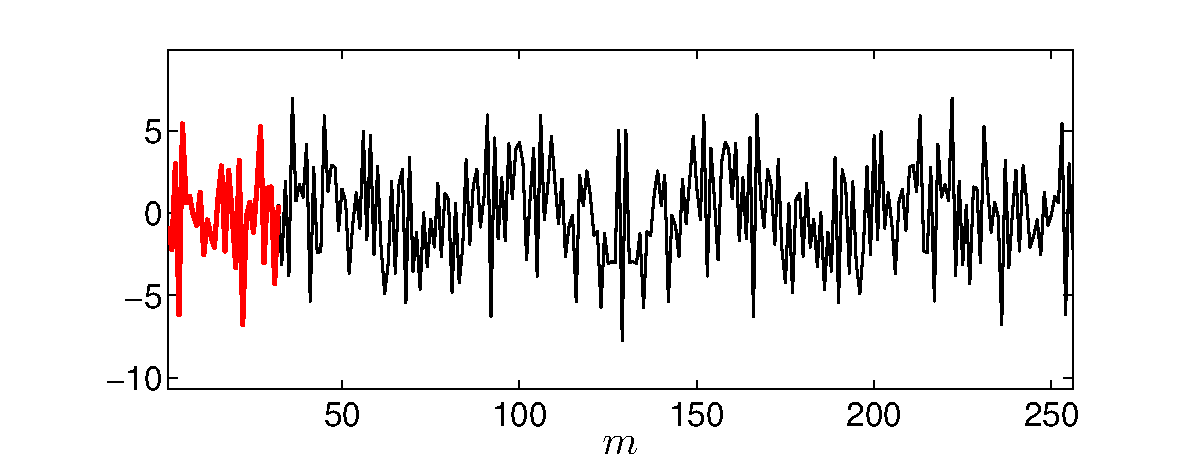
\includegraphics[width=\linewidth]{figures/ft_signal_M_256_N_32_K_16}
\caption{$\Re{\bhx}$ and available $M$ samples}
\end{subfigure}
\\
\begin{subfigure}{.44\textwidth}
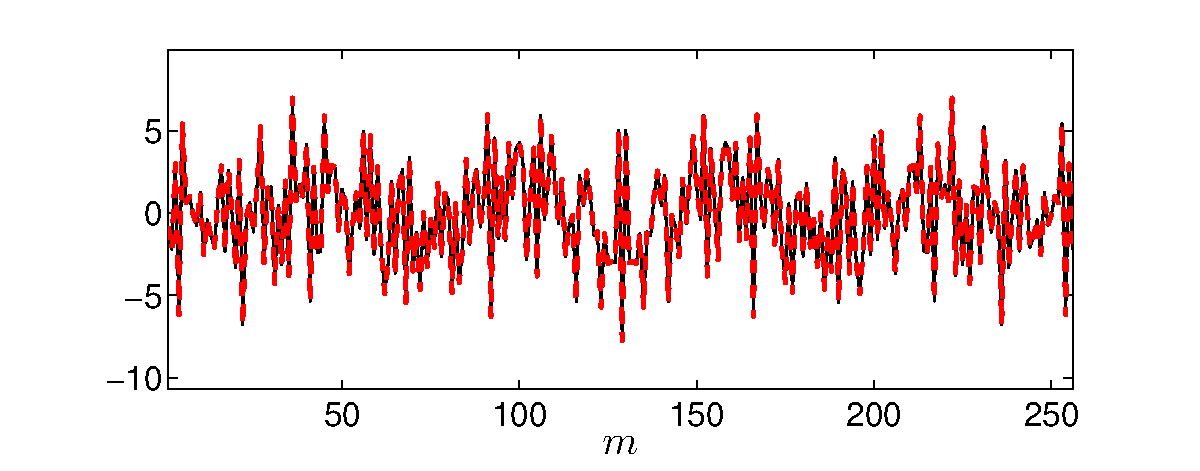
\includegraphics[width=\linewidth]{figures/ft_extrapolate_signal_M_256_N_32_K_16}
\caption{$\Re{\bhx}$ and extrapolated coefficients}
\end{subfigure}
\caption{$N=256$, $M=32$ and $K=16$. (a) Signal with $K=16$ Diracs. (b) Perfect reconstruction
of the signal, in red the original signal and in blue the reconstruction. (c) Real part of the 
Fourier coefficients in black and available samples in red. (d) Real part of the Fourier 
coefficients in black and extrapolated coefficients using the method in Proposition
\ref{prop}, in red.}
\label{fig:signal}
\end{figure}

\begin{figure*}[t]
\centering
% \begin{subfigure}{.3\textwidth}
% \includegraphics[width=\linewidth]{figures/finite_fri_tls_oracle_real_randn_0_M_256_N_64_SNR_5}
% \caption{SNR = 5 dB}
% \end{subfigure}
% \begin{subfigure}{.3\textwidth}
% \includegraphics[width=\linewidth]{figures/finite_fri_tls_oracle_real_randn_0_M_256_N_64_SNR_10}
% \caption{SNR = 10 dB}
% \end{subfigure}
% \begin{subfigure}{.3\textwidth}
% \includegraphics[width=\linewidth]{figures/finite_fri_tls_oracle_real_randn_0_M_256_N_64_SNR_15}
% \caption{SNR = 15 dB}
% \end{subfigure}
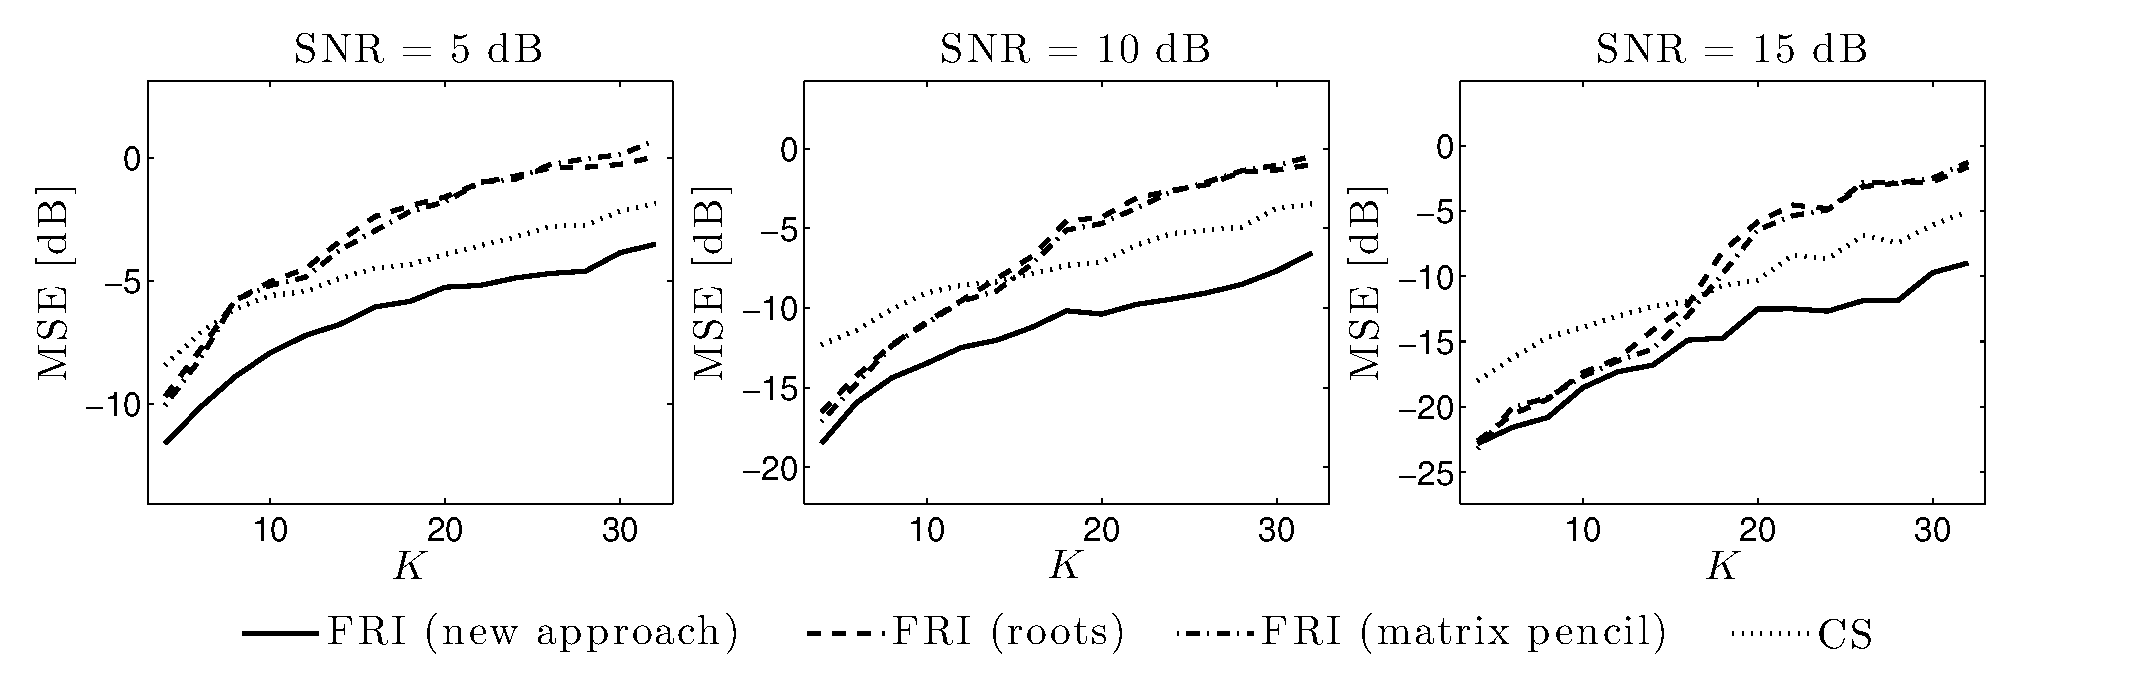
\includegraphics[width=.8\textwidth]{figures/simulation_results_dB}
\caption{Simulation results showing new finite dimensional FRI approach outperforming
traditional FRI methods (root finding of the annihilating filter or matrix pencil) 
and compressed sensing reconstruction. The dimensionality
of the input vector is $N=256$ and the number of available samples is $M=64$. Simulations performed at 
different levels of noise (SNR of 5, 10 and 15 dB) and different levels of sparsity $K$ (horizontal axis).
The vertical axis shows the normalized average value of the MSE of the reconstructed
sparse vector compared to the true $\x$.}
\label{fig:results}
\end{figure*}

\begin{remark}
Proposition \eqref{prop} shows that it is possible to perfectly reconstruct the $K$-sparse
signal $\x$ from the critical number of samples $M=2K$ without having to compute explicitly 
the roots of the annihilating filter. 
% The annihilating filter's coefficients are first obtained
% by building a Toeplitz matrix from samples $\y$ as in \eqref{eq:system}. The $K$-sparse vector
% is then reconstructed by estimating the coefficients of the null space of system \eqref{eq:under_y}. 
\end{remark}

\begin{remark}
Samples in $\y$ correspond to the lower frequencies of $\bhx$, but this can be generalized 
to any $M=2K$ consecutive elements of $\bhx$. Moreover,
due to the periodicity of the DFT the samples only need to be consecutive modulo $(N)$.
\end{remark}

Figure \ref{fig:signal} illustrates the perfect reconstruction of a sparse signal with $K=16$
Diracs. The number of available samples is equal to the number of degrees of freedom of the 
signal: $M=2K=32$. 
The $\beta_l$, $l=1,\ldots,L$ coefficients in the proof of Proposition \eqref{prop} 
correspond to the missing coefficients of the Fourier transform of $\x$ and their real parts
are illustrated in Figure \ref{fig:signal}-(d).


\subsection{Noisy case}

To make the algorithm more robust to noise we have to increase the number of available samples $M$
and apply some denoising algorithm to the samples.
In the presence of noise the Toeplitz matrix $\toe{\y}{K}$ is full rank instead of being rank 
deficient with rank $K$. We first denoise 
vector $\y$ applying an iterative algorithm that finds the closest Toeplitz matrix of rank $K$.
This iterative algorithm is known as Cadzow denoising \cite{cadzow1988} and have been successfully
applied in the FRI context \cite{blu2008}.
% We build a Toeplitz matrix from samples $\y$ wich is closer to a square 
% matrix and we find the closest rank deficient performing a singular value decomposition (SVD)
% and keeping only the $K$ biggest singular values. This new matrix is not Toeplitz anymore, we thus
% force it to be Toeplitz by averaging along the diagonals. This process is repeated until the ratio
% of the singular values is smaller than a threshold.

% We model the observed noise with additive white Gaussian noise:

The annihilating filter is then estimated computing the total least squares (TLS) solution that
minimizes $\norm{\bm{Y}\,\bm{h}}^2$ subject to $\norm{\bm{h}}=1$. In order to reconstruct the sparse vector we
have then to estimate the $\beta_l$ coefficients.
In the noiseless case, the first $M-K$ rows of \eqref{eq:system_beta} are equal to zero, but this 
does not hold when noise is present. We thus have an overdetermined system that we also solve
by computing the TLS solution.
Note that because we have a larger $M$ than the critical value of $2K$, the dimension of the null
space $L=N-M$ is reduced, and thus there are less coefficients $\beta_l$ to be estimated making the 
overall algorithm stable in noisy scenarios.
From the estimated coefficients $\beta_l$ and the available samples $\y$, we build vector $\bhx$ 
with equation \eqref{eq:x_k_null_space}
and apply again the Cadzow denoising algorithm to $\toe{\bhx}{K}$. The sparse vector $\x$ is then obtained
by taking the inverse Fourier transform of $\bhx$.



% --------------
% Fourth section
% --------------

\section{Simulation results}
\label{sec:results}

Figure \ref{fig:results} shows simulations results where the new finite dimensional FRI approach 
outperforms traditional FRI methods and CS reconstruction. 
%For the traditional FRI we have also applied the Cadzow algorithm to denoise 
%the samples. The locations are then obtained from the roots 
%of the annihilating filter and are rounded to nearest integer location or are obtained by 
%applying the matrix pencil method. 
Two different approaches have been tested for the traditional FRI setup.
One approach is to evaluate the annihilating filter polynomial on a grid of $N$ points and estimate
the roots from the local minima of its absolute value. The second approach is to obtain the locations
by applying the matrix pencil method. In both cases, the samples have been first denoised 
applying the Cadzow denoising algorithm.
The CS reconstruction is obtained by applying basis pursuit denoising \cite{chen1998}.
The solution is given by
$\min_{\x\in\C^N} \norm{\x}_1 + (1/2\rho)\,\norm{\y-\D\,\x}_2^2$ and
we have used the YALL1 implementation \cite{zhang2011} with parameter $\rho=10^{-3}$.
We improve the CS solution by picking the $K$ largest values.
For each sparsity level $K$, 10 different distributions for the locations of the Diracs have been uniformly
generated. For each instance of locations the amplitudes of the Diracs are drawn from a Gaussian distribution
with parameters $\mathcal{N} \left(0,1\right)$. Complex noise is added to vector $\y$. The real and imaginary
parts are drawn from $\mathcal{N} \left(0,\sigma\right)$ where
$\sigma$ is adjusted to satisfy the different SNR levels in the measured samples $\y$. 
For each realization of the sparse vector, 100 realizations of noise have been generated. We thus have 1000
realizations for each level of sparsity.

The new finite dimensional FRI method clearly outperforms the other approaches especially in 
high noise scenarios (SNR = 5 dB) and with large values 
of $K$ where the root finding approach becomes more unstable.




% Conclusions and future work
% ---------------------------
\section{Conclusions}
\label{sec:conclusions}

In this paper we have presented a novel method to reconsctruct a finite dimensional
sparse vectors from partial knowledge of its discrete Fourier transform. We have shown
that in the noiseless scenario perfect reconstruction is achieved with the critical 
number of samples. In the noisy case, this method is more stable and outperforms 
traditional FRI approaches and CS because it takes advantage of the fact that the null space
of the underdetermined system is finite dimensional.


\vfill\pagebreak

% Bibliography
% ------------
%\bibliographystyle{IEEEbib.bst}
\bibliographystyle{IEEEtran}
\bibliography{references}


% - end of content
% ------------------------------------------------------------------------------

\end{document}

% - end of document
% ------------------------------------------------------------------------------
